\glsresetall{} 
\chapter{Software Architecture}


\section{POPS Architecture}

The \gls{pops} is made up of several distinct components separated into
services.  Each service has its own Docker5 container. Containers are similar
to virtual machines in that they simulate an operating system but, unlike
virtual machines, they do not simulate the underlying hardware. This makes
containers much more lightweight, while also retaining the benefits of having a
standardized environment where dependencies are packaged with their source
code. Containers make deploying and maintaining \gls{pops} much easier since
installation does not require managing dependencies and tweaking environment
variables. In this way, a \gls{pops} user does not need to be as familiar with
the software as a developer to run it. Each service is its own Python web
server.  In this way, they may be interacted with via a RESTful API. That
being, HTTP requests can be made to retrieve information or perform
calculations. Each service also provides its own automatically generated
documentation that can be accessed through a web browser. This documentation
outlines possible API calls as well as their input and output data formats.
This allows a user to quickly see the capabilities of a service without
accessing the source code. Currently, \gls{pops} has 4 main services; they are
the: Mission Model, Propagator, Database, and Access Time Utilities.  Mission
Model.


\subsection{Mission Model}

The Mission Model service is the service that contains the main logic for most
of \gls{pops}’s functionality and front-end GUI. When a user interacts with
\gls{pops}, they are interacting with the Mission Model service.   Part of the
Mission Model service supports the 3D Earth visualization tool, CesiumJS4.
CesiumJS can display time-dynamic, geospatial information on a webpage.  With a
custom-made Cesium handler class, \gls{pops} can visualize: the Earth,
spacecraft, their orbits, ground stations, and can draw polygons on the Earth.
In addition to displaying information, the handler class also enables a user to
make changes in the viewer which are then reflected in \gls{pops} itself. The
mission model service has many other features including: database management,
opportunity filtering, and scheduling. These features will be discussed in the
WORKFLOW section.  

\subsection{Propagator}

The Propagator service handles ephemeris generation for \gls{pops}.
Ephemerides are a crucial component for every subsequent step along the
planning process so it is essential that they are well formed. Consolidating
ephemeris generation for the entire tool ensures that only one area of the code
needs to be developed and validated.

Currently, the main method of orbital propagation for \gls{pops} is with the
\gls{sgp} model series of algorithms, specifically SGP4/SDP4 referred to as
just ‘SGP4’. SGP4 is an analytical method of approximating orbital state
vectors at corresponding epochs in the \gls{teme} \gls{eci} coordinate frame,
given a NORAD \gls{tle}.  \gls{tle}s are readily provided by the United States
Space Force through Space-Track6 or CelesTrak7. The \gls{teme} coordinate frame
is not particularly useful so part of the Propagator service’s purpose is
transforming the orbit vectors into a coordinate system required by other parts
of \gls{pops}.  Currently, the two possible output reference frames are the
\gls{gcrs}, which is an \gls{eci} reference frame, and the \gls{wgs}, which is
an \gls{ecef} reference frame.  Depending on the application, it is sometimes
useful to use \gls{eci} or \gls{ecef} reference frames, so both are made
available by the service.  Given a \gls{tle}, a time range, a step size, and a
coordinate system, the Propagator service generates an Ephemeris for the
provided time range in a variety of output formats.

It is very easy to generate Ephemeris data. What is difficult is validating it.
The benchmark for validation is \gls{stk} since it has its own SGP4 ephemeris
generation capabilities. If operators did not use POPS, their best alternative
would be to set up scenarios manually in \gls{stk}. As such, using it as ground
truth is valid in this case. Both \gls{stk} and the \gls{pops} implementation
of SGP4 us the same source8: Revisiting Spacetrack Report \#39. As such, they
should provide the same results. One difference to note is that \gls{stk} uses
the \gls{icrf} \gls{eci} coordinate system but the propagator service uses
\gls{gcrf}.  This difference is acceptable since these reference frames are
approximately identical10. The procedure for validating the Propagator service
was first to select a \gls{tle}, a time range, a time step, and a coordinate
system.  Next was to generate Ephemerides from \gls{stk} and the propagation
service.  Finally, the results were compared. One such comparison can be seen
in Figure \ref{fig:stk_py}. Here, the peak position residual was 0.37mm for the position along
the x-axis. The main purpose of this exercise is to ensure that the Python
libraries are being used correctly and that their output data is acceptable.
From this result, it is clear that the methods are identical and the difference
was most likely due to slight implementation differences. 

\begin{figure} 
    \centering
    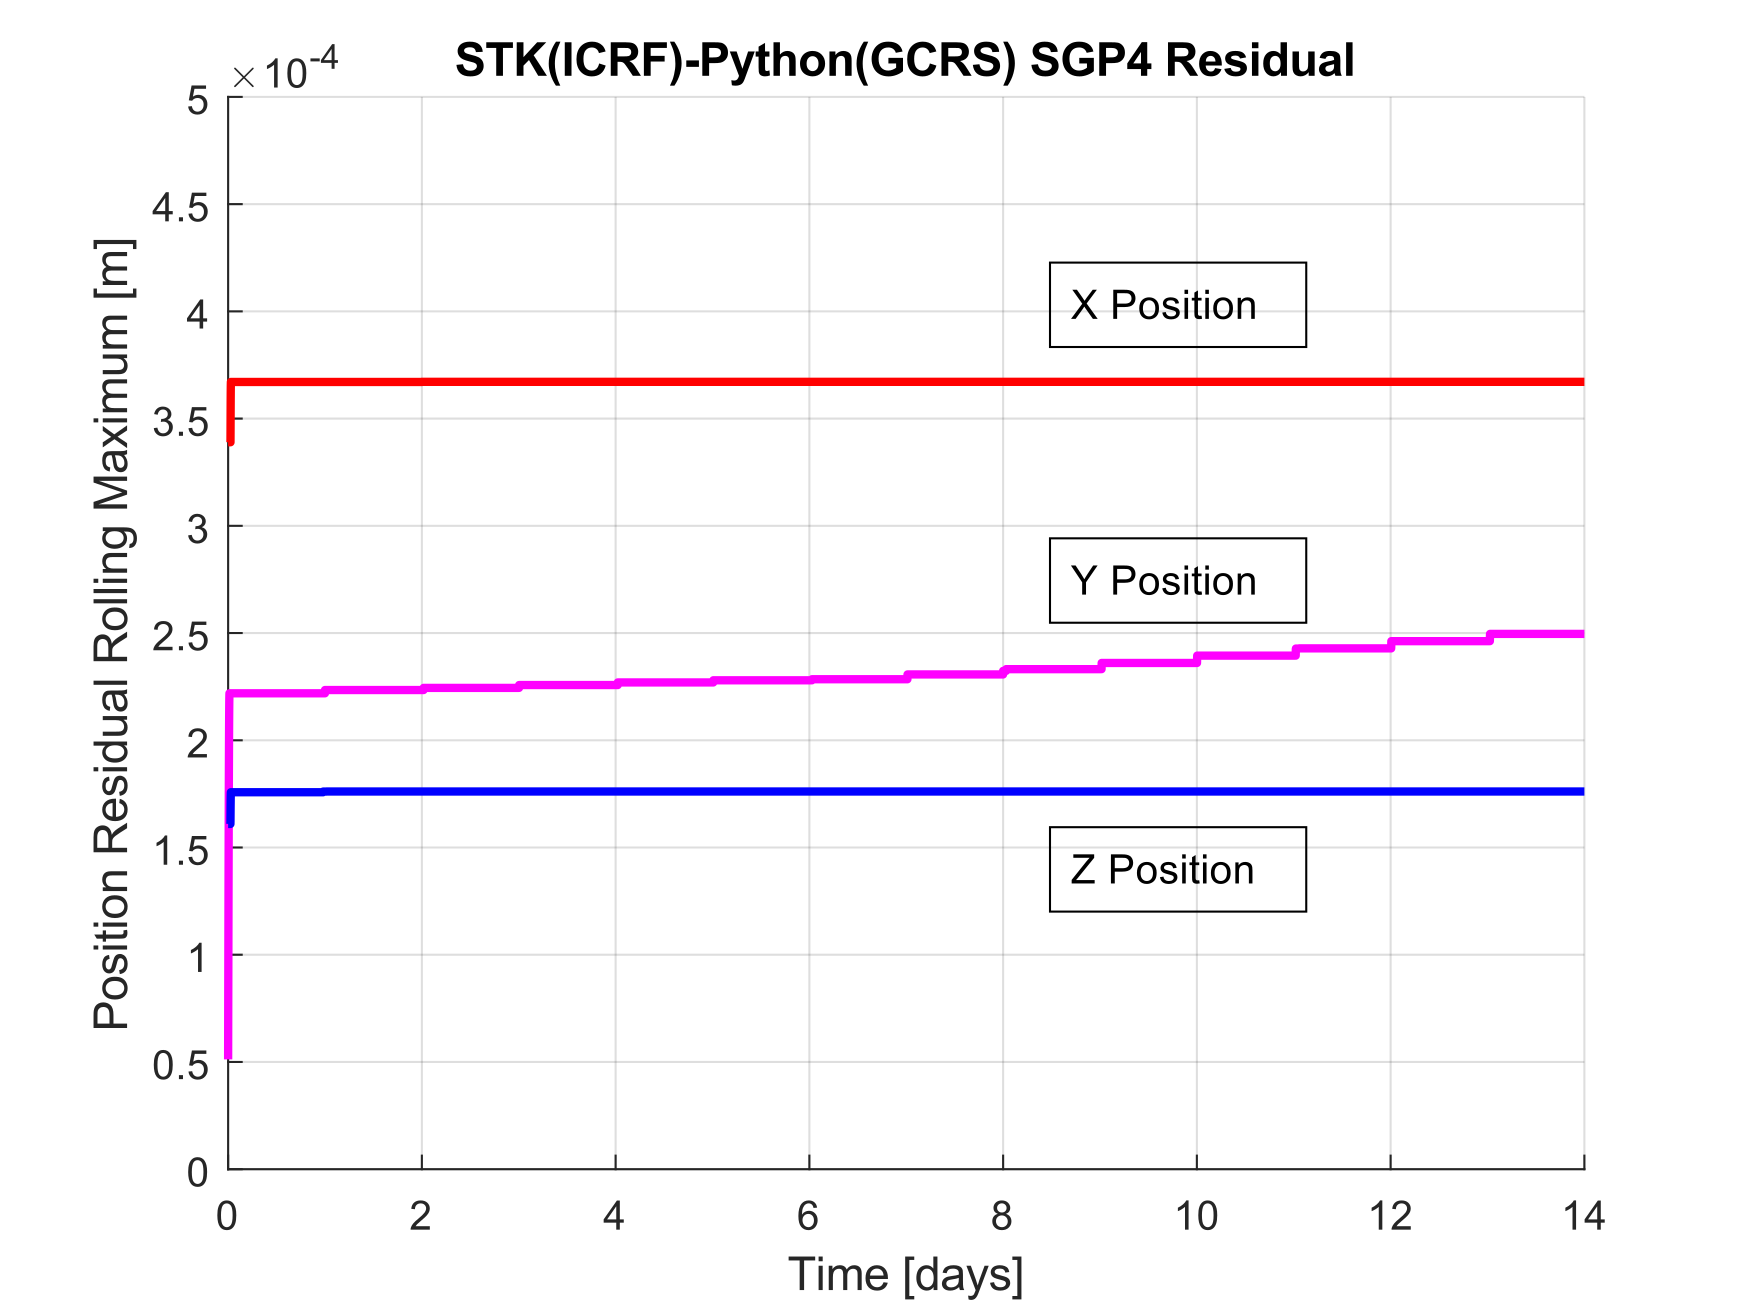
\includegraphics[width=0.7\textwidth]{STK_PY_residual-2.png} 
    \caption{Residual Difference \gls{stk} vs. Python}
    \label{fig:stk_py} 
\end{figure}

Part of the benefit of having the Propagator as its own service is that if a
more accurate algorithm is desired for orbital propagation, only the Propagator
service needs to be changed and the rest of \gls{pops} can be left as is.


\subsection{Access Time Utilities}

The ATU service provides the basic building blocks for
constraining observation opportunities. These can be added to depending on a
mission’s need. The \gls{atu} service currently supports calculating: ground station
access times, swath generation, horizon swath generation, and polygon
intersection with a swath. These will be discussed in detail in their own
section.  


\subsection{Database}

\gls{pops} must be able to retain information, even if it is
shut down or moved somewhere else. It is also necessary that data be stored
such that it does not sit in RAM. For this reason, an SQL database service is
included. It stores all the data necessary for \gls{pops} to function. This
includes but is not limited to satellite information, \gls{tle}s, current and
previous plans, ephemeris data, observation opportunity data, and planned
observations. Using an SQL database allows for effective data storage and
access. There are also no read or write restrictions on an SQL database so data
can be accessed simultaneously by multiple users or services.





\section{Access Time Utilities}


The Access Time Utilities are the fundamental components that enable POPS to be
a planning software. They form the basic building blocks for constraining
observation opportunities. Additional utilities can be added depending on a
mission’s need. The following sections discuss the baseline functionality that
has currently been implemented.


\subsection{Ground Access Utility}

A Ground Access is defined as the time interval during which a satellite can
establish contact with a ground station. A ground station is a point on the
Earth’s surface, identified with geodetic latitude-longitude-altitude
coordinates and an elevation mask. An elevation mask is the angle above the
horizon, at the ground station’s position, at which the satellite can be
considered visible by the ground station. Calculating the ground access for
satellites on a mission is a fundamental task in operations planning. These
time intervals dictate the opportunities for data downlink, command uplink, and
any other communication between the ground segment and satellite. 

The simplest way to compute ground access involves propagating the orbit of a
satellite and checking, at every time step, the position of the satellite
relative to the ground station and testing whether the relative position is
above the elevation mask. While this method is trustworthy and capable of
returning accurate results, its reliance on iterating over an entire satellite
orbit input typically yields a long runtime. This is particularly evident in
the case where a mission has multiple ground stations, multiple satellites, or
a short propagator timestep. The computation time drawback motivates the use of
other algorithms that can determine ground access more efficiently. 

There have been a plethora of papers published on the subject of efficiently
computing ground access over the years. Early work includes Lawton’s
development of a method for calculating ground access for low-eccentricity
satellite orbits by leveraging the Fast Fourier Transform to quickly find a
ground access11. Alfano et al.12 use another technique known as parabolic
blending for constructing the visibility function and finding ground access.
While POPS currently utilizes the simplest method for calculating ground
access, the method that is selected for future implementation is that of Han et
al.13, which uses a self-adaptive interpolation technique to approximate the
waveform of the visibility function. The advantage of this method is its
suitability for all orbit types and orbit propagators, which allows the methods
employed by POPS to generalize for any mission orbit definition. 


\subsection{Swath Utility} 

As discussed in the Terminology section, the concept of an access swath is
defined as a time-series of access regions as a satellite orbits the Earth.
Within \gls{pops}, a swath is represented through a closed curve that describes
the boundary of the cumulative access region of a sensor’s \gls{for} over a
time interval. The process for calculating a swath boundary from an input
ephemeris is described here. 



\subsection{Swath Intersection Utility}

Swath intersection is an important operation for determining what part of a
specified region is observable by a satellite sensor during some time interval.
Regions are polygons on the Earth’s surface whose vertices are oriented
counter-clockwise. The edge between two consecutive vertices is the great
ellipse arc connecting both points. Swaths are also approximated as polygons
provided that the timestep is small enough. The edge between two swath boundary
points being a great ellipse arc is assumed to be a sufficient approximation. 

Polygon clipping techniques are used to find the area of intersection between a
swath and a polygon. First, the swath and polygon vertices are transformed into
2D coordinates. The 2D projection used involves defining a plane that is
tangent to some point on the Earth’s surface. To project a point on the Earth’s
surface to this plane, a vector is drawn from the centre of the Earth towards
the point (its \gls{ecef} coordinates), and the vector is extended towards the
point of intersection of the plane. This type of projection is commonly known
as the Gnonomic projection; its advantage with respect to the polygon clipping
operation is that great ellipse arcs are projected as straight lines. This
means classical 2D polygon clipping techniques can be applied to polygons drawn
on the Earth’s surface. So long as the swath and polygon occupy one hemisphere
of the Earth’s surface, the projection will accurately represent the points of
intersection of the swath and polygon, and any polygon clipping technique can
be applied. 




